\section{Mealy machines with timers}

\subsection{Definition and timed semantics}
We assume an infinite set $X = \{ x_1, x_2, x_3,\ldots \}$ of {\em timers}.
Let $\toevents$ be the set of {\em timeout events} of the form
$\toevent{x}$ for $x \in X$.
For a set $I$, let $\extinputs$ be $I \cup \toevents$.
%
We write $A \hookrightarrow B$ for the set of partial functions from $A$ to $B$.
With $f \lceil A$ we denote the restriction of function $f$ to $\domof{f} \cap A$.
%For arbitrary functions $f$ and $g$, $f [g]$ is the function with domain $\domof{f}$ that behaves like $f$
%on $\domof{f} \setminus \domof{g}$ and like $g$ on $\domof{f} \cap \domof{g}$.
We write $\finitesubsets{A}$ for the set of finite subsets of set $A$.

\begin{definition}
\label{def:MMT}
A \emph{Mealy machine with timers (MMT)} is a tuple
\\
$\M = (I, O, Q, q_0, \vars, \delta, \lambda, \remap)$, where
\begin{itemize}
\item
$I$ and $O$ are finite sets of input events and output events, respectively,
\item
$Q$ is a finite set of states,
with
$q_0 \in Q$ the initial state,
\item
$\vars: Q \rightarrow \finitesubsets{X}$, with $\varsof{q_0} = \emptyset$,
\item
$\delta: Q \times \extinputs \hookrightarrow  Q$ is a transition function,
%with $\delta(q,i)$ defined iff $q \in Q$ and $i \in I \cup \{ \toevent{x} \mid x \in \varsof{q} \}$, 
\item
$\lambda: Q \times \extinputs \hookrightarrow O$ is an output function, 
\item
$\remap : Q \times \extinputs \hookrightarrow (X \hookrightarrow \natplus)$ is a timer update function.
\end{itemize}
Let $q \in Q$, $i \in \extinputs$, $q'=\delta(q,i)$ and $\rho=\remap(q,i)$. 
We require that $\varsof{q'} \setminus \varsof{q} \subseteq \domof{\rho} \subseteq\varsof{q'}$. 
When timer $x$ expires it is either stopped or restarted:
if $i=\toevent{x}$, for some $x$, then $x \not\in \varsof{q'} \setminus \domof{\rho}$.
%
We also require that input events are always enabled and timeout events are enabled
for timers that are active in the current state:
$\delta(q,i)$, $\lambda(q,i)$ and $\pi(q,i)$ are defined iff either
$i \in I$ or $i=\toevent{x}$, for some $x \in\varsof{q}$.
We write $q \xrightarrow{i/o,\rho} q'$ if $\delta(q,i) = q'$, $\lambda(q,i)= o$ and $\remap(q,i) = \rho$.
\end{definition}
Update function $\remap$ determines how timers are affected when an event occurs. Suppose $q \xrightarrow{i/o,\rho} q'$.
Basically, four things may happen:
%\marginpar{Add Venn diagram to illustrate situation?}
%Let $q \in Q$, $i \in \extinputs$, $\delta(q,i)=q'$ and $\remap(q,i)=\rho$.
\begin{enumerate}
\item
If $x \in\varsof{q} \setminus \varsof{q'}$ then input $i$ \emph{stops} timer $x$.
\item
If $x \in \varsof{q'} \setminus \varsof{q}$ then $i$ \emph{starts} timer $x$ with value $\rho(x)$.
\item
If $x \in \varsof{q} \cap \domof{\rho}$ then $i$ \emph{restarts} timer $x$ with value $\rho(x)$.
\item
Finally, if $x \in \varsof{q'} \setminus \domof{\rho}$ then timer $x$ is \emph{unaffected} by $i$.
\end{enumerate}

\paragraph{Semantics.}
We define the semantics of an MMT $\M = (I, O, Q, q_0, \vars, \delta, \lambda, \remap)$ 
via an infinite state transition system that describes all possible
configurations and transitions between them.
A \emph{valuation} is a partial function
$\tvals : X \hookrightarrow \realsplus$, defined on a finite subset of $X$, that assigns nonnegative real numbers as values to timers.
We write $\Vals{Y}$ for the set of valuations with domain $Y \subseteq X$.
A \emph{configuration} of an MMT is a pair $(q,\tvals)$, where $q \in Q$ is a state and $\tvals\in\Vals{\varsof{q}}$ is a valuation.
The \emph{initial configuration} is the pair $(q_0, \tvals_0)$, where $\tvals_0$ is the empty function.
Valuations and configurations can be modified by the occurrence of input and timeout events, and by
the occurrence of delays.
If $\tvals$ is a valuation in which all timers
have a value of at least $d$, then $d$ units of time may pass. As a result of this delay the value of all the timers is decremented by $d$.
Formally, for $\tvals, \tvals'$ valuations and $d \in \delays$, we define a delay transition relation by: $\tvals \xrightarrow{d} \tvals'$ iff
\[
\domof{\tvals} = \domof{\tvals'} \wedge \forall x \in\domof{\tvals} : \tvals'(x) = \tvals(x) - d .
\]
If the current valuation is $\tvals$, then timeout event $\toevent{x}$ may occur only if $\tvals(x)=0$.
If an input or a timeout event occurs, $\tvals$ is updated as specified by update function $\rho$.
The values of timers that are not affected by $\rho$ remain unchanged.
Formally, for $\tvals, \tvals'$ valuations, $i \in \extinputs$, $o \in O$ and $\rho \in X \hookrightarrow \natplus$,
we define a discrete transition relation by: $\tvals \xrightarrow{i/o, \rho}  \tvals'$ iff
\begin{eqnarray*}
&& \domof{\tvals'} \setminus \domof{\tvals}  \subseteq \domof{\rho} \subseteq \domof{\tvals'} ~ \wedge\\
&& [\forall x \in\domof{\tvals'} : \tvals'(x) = \mbox{ if } x \in\domof{\rho} \mbox{ then } \rho(x) \mbox{ else } \tvals(x)] ~ \wedge\\
%More concise but harder to understand:
%&& \tvals' =  \tvals'[\tvals][\rho] ~ \wedge \\
&& \forall x \in X : i=\toevent{x} \Rightarrow (\tvals(x) = 0 \wedge x \not\in\domof{\tvals'} \setminus \domof{\rho}).
\end{eqnarray*}
%Condition $\tvals' =  \tvals'[\tvals][\rho]$ expresses that $\tvals'$ is obtained by giving variables
%in $\domof{\rho}$ the value specified by $\rho$, and all remaining variables the value specified by $\tvals$.
Transition relations $\xrightarrow{d}$ and $\xrightarrow{i/o, \rho}$ can be easily lifted to configurations.
For all configurations $(q, \tvals)$, $(q', \tvals')$ of an MMT $\M$,
\[
\frac{q = q' \quad \tvals \xrightarrow{d} \tvals'}{(q,\tvals) \xrightarrow{d} (q',\tvals')}
\quad\quad
  \frac{q \xrightarrow{i/o,\remapinst} q' \quad \tvals \xrightarrow{i/o, \rho} \tvals'}{(q,\tvals) \xrightarrow{i/o} (q',\tvals')}
\]
A \emph{timed run} of $\M$ over $w$ is a sequence 
\begin{eqnarray*}
\alpha & = & C_0 \xrightarrow{d_1} C'_0 \xrightarrow{i_1/o_1} C_1 \xrightarrow{d_2} 
%C'_1 \xrightarrow{i_2/o_2} C_2 
\cdots
\xrightarrow{d_k} C'_{k-1} \xrightarrow{i_k/o_k} C_{k}
\end{eqnarray*}
of transitions between configurations $C_j, C'_j$ of $\M$, where $C_0$ is the initial configuration.
%Note that, since MMTs are deterministic (if we allow to observe the
%identities of timers in timeout events),
%for each timed word $w$ there exists at most one run over $w$.
A \emph{timed word} over inputs $I$ and outputs $O$ is a sequence
\begin{eqnarray*}
w & = &  d_1 ~ i_1 ~ o_1 ~ d_2 ~ i_2 ~ o_2 \cdots d_k ~ i_k ~ o_k,
\end{eqnarray*}
where $d_j \in \delays$, $i_j \in I \cup \{ \mathit{to} \}$, and $o_j \in O$.
To each timed run $\alpha$ we associate a \emph{timed word} by forgetting the configurations and the timers
in timeout events:
\begin{eqnarray*}
\timedword(\alpha) & = & d_1 ~ i'_1 ~ o_1 ~ d_2 ~ i'_2 ~ o_2 \cdots d_k ~ i'_k ~ o_k,
\end{eqnarray*}
where for all  $j$,
\begin{eqnarray*}
i'_j  & = &   \left\{ \begin{array}{ll}
i_j & \mbox{if } i_j \in I,\\
\mathit{to} & \mbox{if } i_j \in \toevents.
\end{array} \right.
\end{eqnarray*}
The idea is that timeouts cannot be observed directly. 
However, when we observe an output that is not triggered by an input, we may
conclude that a timeout occurred. But in general we do not know which timer expired.

We say $w$ is a timed word of $\M$ if $\M$ has a timed run $\alpha$ with $w = \timedword(\alpha)$.
%
Two MMTs $\M$ and $\N$ with the same sets of inputs are \emph{timed equivalent}, denoted $\M \approx_{\mathit{timed}} \N$, iff 
they have the same sets of timed words.

\iflong
\paragraph{Remark.}
In our semantics we assume that discrete transitions occur instantaneously and take no time. In applications, however, i/o interactions
often take a significant amount of time. In \cite{SHV16}, for instance, a case study of an interventional X-ray system is
described in which a single i/o interaction may take several seconds. If it is important to model such delays
explicitly, this can be done within the MMT framework by splitting a transition with input $i$ and output $o$ into
a pair of consecutive transitions: a first transition with input $i$ and some default output $\Lambda$ that starts
a timer $x$, and a second transition in which $x$ times out and output $o$ is produced.
If inputs arrive in the newly introduced intermediate state, these may either be ignored, buffered or forbidden
(via a transition to some designated error state).
Note that $\Lambda$ corresponds to the \emph{absence} of an observable output. For inputs $i \in I$ this is fine: if such
an input does not trigger an observable output then we just assume that the output event is $\Lambda$. We do not allow
$\Lambda$ as output event in timeout transitions $\toevent{x}$: since timeout events themselves are not observable, we can ony observe their occurrence indirectly through the observable output that they trigger.

\paragraph{Remark.}
Note that we assume that in a timed run each discrete transition is preceded by a nonzero delay.
The idea that multiple consecutive discrete transitions may occur in zero time is a useful abstraction in synchronous
programming and in the theory of timed automata, but nonzero delays form
a crucial requirement for the learning algorithm that we present in this paper.

Disallowing zero delays creates certain complications that we have to deal with. The simple MMT of Figure~\ref{fig:timelock}, for instance,
may reach a timelock following the timed word $1 ~ i ~ o ~ 1 ~ i ~ o$: at this point timer $x$ has value $0$, but no timeout is enabled since first a nonzero amount of time has to elapse, which is not possible since then $x$ would become negative.
\begin{figure}[ht]
\begin{center}
\begin{tikzpicture}[->,>=stealth',shorten >=1pt,auto,node distance=2.5cm,main node/.style={circle,draw,font=\sffamily\large\bfseries}]
  \node[initial, state] (1) {$q_0$};
  \node[state] (2) [right of=1] {$q_1$};
  \node[state] (3) [right of=2] {$q_2$};
  
  \path[every node/.style={font=\sffamily\scriptsize}]
    (1) edge node {$i/o$, $~x:=1$} (2)  
    (2) edge  node {$\toevent{x}/o'$} (3)
        edge  [loop below] node {$i/o$} (2)
    (3) edge  [loop below] node {$i/o$} (4);
\end{tikzpicture}
\caption{An MMT with a timelock}
\label{fig:timelock}
\end{center}
\end{figure}
Once solution would be to disable inputs in $I$ whenever a timer has become $0$. 
In Section~\ref{section untimed semantics}, we will elaborate
a different approach in which we only consider runs in which no ``races'' occur. This eliminates the problematic
behavior of the above MMT in which there is a race between the second $i$ event and the timeout.
\fi

\paragraph{Experiments and nondeterminism.}
Due to our assumption that we cannot observe the identity of a timer in a timeout event, an MMT may exhibit nondeterministic
behavior: even if we offer exactly the same inputs at exactly the same time, different outputs may occur in different runs. 
The MMT of Figure~\ref{fig:nondeterminism} (top), for instance, has timed words
$1 ~ i ~ o ~ 1 ~ \mathit{to} ~ o'$ and $1 ~ i ~ o ~ 1 ~ \mathit{to} ~ o''$.
(For clarity, we omit some self-loop transitions.)
\begin{figure}[ht]
\vspace{-1em}
\begin{center}
\begin{tikzpicture}[->,>=stealth',shorten >=1pt,auto,node distance=1.8cm,main node/.style={circle,draw,font=\sffamily\large\bfsthe name of the eries}]
  \node[initial, state] (1) {$q_0$};
  \node[state] (2) [below of=1] {$q_1$};
  \node[state] (3) [right of=2] {$q_3$};
  \node[state] (4) [left of=2] {$q_2$};

  \path[every node/.style={font=\sffamily\scriptsize}]
    (1) edge node {$i/o$, $~x:=1$, $y:=1$} (2)  
    (2) edge  node {$\toevent{x}/o'$} (3)
     edge  node {$\toevent{y}/o''$} (4);
\end{tikzpicture}
\begin{tikzpicture}[->,>=stealth',shorten >=1pt,auto,node distance=2.2cm,main node/.style={circle,draw,font=\sffamily\large\bfseries}]
  \node[initial, state] (1) {$q_0$};
  \node[state] (2) [right of=1] {$q_1$};
  \node[state] (3) [right of=2] {$q_2$};

  \path[every node/.style={font=\sffamily\scriptsize}]
    (1) edge [text width=1cm] node {$i/o$\\ $x:=2$} (2)  
    (2) edge [text width=1cm] node {$i/o$\\ $y:=1$} (3)
      edge  [loop below] node {$\toevent{x}/o$, $~x:=2$} (2)
   (3) edge  [loop below] node {$\toevent{x}/o'$, $x:=1$} (3)
   edge  [loop above] node {$\toevent{y}/o''$, $y:=1$} (3);
\end{tikzpicture}
\caption{MMTs with ``uncontrollable'' and ``controllable'' nondeterminism}
\label{fig:nondeterminism}
\end{center}
\end{figure}

%In order to rule out this type of nondeterminism, it is not enough to require that the timer update functions are injective,
%that is, it is not allowed to assign the same value to multiple timers in a single transition.
%This is illustrated by the MMT of Figure~\ref{fig:nondeterminism2}, which accepts both the timed words
%$1 ~ i ~ o ~ 1 ~ \mathit{to} ~ o'~ 1 ~ \mathit{to} ~ o'$ and $1 ~ i ~ o ~ 1 ~ \mathit{to} ~ o' ~ 1 ~ \mathit{to} ~ o''$.
%\begin{figure}[ht]
%\begin{center}
%\begin{tikzpicture}[->,>=stealth',shorten >=1pt,auto,node distance=2.5cm,main node/.style={circle,draw,font=\sffamily\large\bfseries}]
%  \node[initial, state] (1) {$q_0$};
%  \node[state] (2) [below of=1] {$q_1$};
%  \node[state] (4) [left of=2] {$q_2$};
%
%  \path[every node/.style={font=\sffamily\scriptsize}]
%    (1) edge node {$i/o$, $~x:=1$, $y:=2$} (2)  
%    (2) edge  node {$\toevent{y}/o''$} (4)
%      edge  [loop right] node {$\toevent{x}/o'$, $~x:=1$} (2);
%\end{tikzpicture}
%\caption{Another MMT with nondeterministic behavior}
%\label{fig:nondeterminism2}
%\end{center}
%\end{figure}
%
The nondeterminism of the MMT of Figure~\ref{fig:nondeterminism} (left)
%and \ref{fig:nondeterminism2} 
is ``uncontrollable'' and occurs after any (nonempty) input sequence.
Figure~\ref{fig:nondeterminism} (bottom) gives an example of an MMT that exhibits nondeterminism when the second input occurs \emph{exactly} one time unit after the first input: the MMT has timed words
$7 ~ i ~ o ~ 1 ~ i ~ o ~ 1 ~ \mathit{to} ~ o'$ and $7 ~ i ~ o ~ 1 ~ i ~ o ~ 1 ~ \mathit{to} ~ o''$.
This type of nondeterminism is ``controllable'' and will not occur if we carefully
select the timing of inputs.

Let us formalize these ideas.
A \emph{timed input word} is a sequence
$u = d_1 ~ i_1 \cdots d_k ~ i_k ~ d_{k+1}$, where $d_j \in \delays$ and $i_j \in I$, for all $1 \leq j \leq k$,
and $d_{k+1} \in \realsplus$.
A timed input word describes an experiment that may be carried out on an MMT in which we
provide a series of inputs at specific times, and observe the outputs that occur in response to these inputs up to time $\sum_{j=1}^{k+1} d_j$.
%
We associate a timed input word $\timedinputword(w)$ to each timed word $w$ by 
removing the outputs events, 
removing the occurrences of $\mathit{to}$, 
replacing consecutive numbers by their sum, 
and possibly placing $0$ at the end of the sequence.
Thus, for instance,
$\timedinputword (7 ~ i ~ o ~ 1 ~ i ~ o ~ 1 ~ \mathit{to} ~ o') = 7 ~ i ~ 1 ~ i ~ 1$ and
$\timedinputword (3 ~ i_1 ~ o_1 ~ 1.1 ~ i_2 ~ o_2 ~ 2 ~ \mathit{to} ~ o_3 ~ 2.1 ~ i_4 ~ o_4) = 3 ~ i_1 ~ 1.1 ~ i_2 ~ 4.1 ~ i_4 ~ 0$.
%
If $u$ and $u'$ are timed input words, then we write $u \propto u'$ if $u$ and $u'$ are equal, except that the final delay of $u$ is less or equal than the final delay of $u'$.
For any timed input word $u$ over $I$,  there exists a maximal timed word $w$ of $\M$ such that $\timedinputword(w) \propto u$.
We call $w$ an \emph{outcome of running experiment} $u$ on $\M$.
In general, outcome $w$ is not uniquely determined, and thus an MMT may exhibit nondeterminism. 
In the example of Figure~\ref{fig:nondeterminism} (bottom), for instance, experiment $7 ~ i ~ 1 ~ i ~ 1$ has outcomes
$7 ~ i ~ o ~ 1 ~ i ~ o ~ 1 ~ \mathit{to} ~ o'$ and  $7 ~ i ~ o ~ 1 ~ i ~ o ~ 1 ~ \mathit{to} ~ o''$.

We call timed input word $u$ \emph{transparent} if the fractional part of the absolute times of occurrence of
all the inputs are different. A timed word $w$ is transparent iff $\timedinputword(w)$ is transparent.
If $u$ is transparent, there is a unique outcome of running experiment $u$ on $\M$.
\todofv{clarify this section}
%\iflong
%Note that the first input occurs at time $3$, the second at time $4.1$, and the third at time $8.2$.
%Thus the fractional part of the times of the inputs are different. In fact, 
%\fi
\subsection{A timed MAT framework for learning MMTs}
We now propose an instance of Angluin's MAT framework for Mealy machines with timers.
In our setting, illustrated in Figure~\ref{fig timed MAT}, the teacher knows an MMT $\M$.
Initially, the learner only knows the set $I$ of inputs of $\M$.
The learner may perform experiments (membership queries, MQ) to learn about the
timed words of $\M$, and  pose equivalence queries (EQ) to find out whether a constructed hypothesis is correct.

\begin{figure}[h]
\begin{center}
 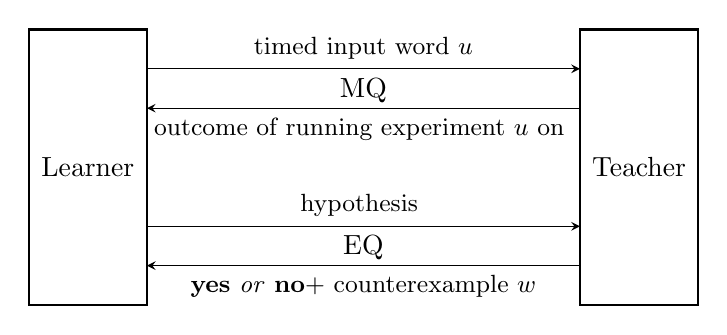
\begin{tikzpicture}[>=stealth]
            \draw [thick] (0,0) rectangle (1.5,3.5) node[midway] {Learner};
            \draw [thick] (7,0) rectangle (8.5,3.5) node[midway] {Teacher};
            %\draw [thick] (7,0) rectangle (8.5,3.5) node[midway,below] {(knows $\M$)};
            \draw [->] (1.5,3) -- (7,3) node[midway,below] {MQ};
            \draw (1.5,3) -- (7,3) node[midway,above] {\small timed input word $u$};
            \draw [<-] (1.5,2.5) -- (7,2.5) node[midway,below] {\small outcome of running experiment $u$ on $\M$};
            \draw [->] (1.5,1) -- (7,1) node[midway,below] {EQ};
            \draw (1.5,1) -- (7,1) node[midway,above] {\small hypothesis $\CH$};
            \draw [<-] (1.5,0.5) -- (7,0.5) node[midway,below] {\small {\bf yes} \emph{or} {\bf no}+ counterexample $w$};
        \end{tikzpicture}
\end{center} 
\caption{A timed MAT framework}
\label{fig timed MAT}
\end{figure}

\paragraph{Membership queries.}
With a \emph{membership query}, the learner asks what the output is in response to a timed input word $u$ over $I$. 
The teacher answers with a maximal timed word $w$ of $\M$ such that $\timedinputword(w) \propto u$.


\paragraph{Equivalence queries.}
With an \emph{equivalence query}, the learner asks if a hypothesized MMT $\CH$ is correct, that is, 
whether $\CH \approx_{\mathit{timed}} \M$.
The teacher answers \emph{yes} if this is the case. Otherwise she answers \emph{no} and supplies a
\emph{counterexample}: a transparent timed word $w$ of $\M$ that is not a timed word of $\CH$.
(We will prove in Lemma~\ref{not timed} that such a timed word always exists.)

\vspace{0.5em}
\noindent
The main result of this paper is an algorithm that allows the learner to learn an MMT $\CH$ that is timed equivalent to
$\M$ via a finite number of membership and equivalence queries. \todofv{Point out restrictions on MMTs (only one timer set per transition, no ghost timers)}

\subsection{Timed and untimed runs and behaviors}
In order to present our algorithm, we need to define a number of abstractions of timed runs.
Configurations consists of pairs of states and timer valuations. This means that there are two natural abstractions of
timed runs: an abstraction $\untime$ that forgets all timing information and keeps the transitions of the MMT, 
and an abstraction $\beh$ that forgets information on states and preserves the timing information.
When we compose these abstractions we obtain \emph{untimed behaviors} in which only information about inputs, outputs,
updates and active timers is preserved.
The abstractions commute, $\beh(\untime(\alpha))=\untime(\beh(\alpha))$, and play a key role in
the technical development of this paper.
%
Formally, an \emph{untimed behavior} over inputs $I$ and outputs $O$ is a sequence 
\begin{eqnarray*}
\beta & = & X_0 \xrightarrow{i_1/o_1, \rho_1} X_1  \cdots \xrightarrow{i_k/o_k, \rho_k} X_{k},
\end{eqnarray*}
where $X_0 \subseteq X$ and, for each $j>0$,  $i_j \in \extinputs$, $o_j \in O$, $\rho_j \in X \hookrightarrow \natplus$, and
 $X_j \setminus X_{j-1}  \subseteq \domof{\rho_j} \subseteq X_j \subseteq X$.
Moreover, if $i_j = \toevent{x}$, for some $j>0$, then $x \in X_{j-1}$ and $x \not\in X_j \setminus \domof{\rho_j}$.
%
An \emph{untimed run} of an MMT $\M$ is a sequence
\begin{eqnarray*}
\gamma & = & q_0 \xrightarrow{i_1/o_1, \rho_1} q_1   \cdots \xrightarrow{i_k/o_k, \rho_k} q_k
\end{eqnarray*}
of transitions of $\M$ that starts with the initial state $q_0$. 
To each untimed run $\gamma$ we associate an untimed behavior by replacing all
states by their sets of timers:
\begin{eqnarray*}
\beh(\gamma) & = & \vars(q_0) \xrightarrow{i_1/o_1, \rho_1} \vars(q_1)  \cdots \xrightarrow{i_k/o_k, \rho_k} \vars(q_k).
\end{eqnarray*}
We say that $\beta$ is an untimed behavior of $\M$ if $\M$ has an untimed run $\gamma$ with $\beh(\gamma) = \beta$.
Note that the initial timer set of an untimed behavior of $\M$ is empty.
%
A \emph{timed behavior} over inputs $I$ and outputs $O$ is an alternating sequence
\begin{eqnarray}
\label{timedbehavior}
\sigma & = & \tvals_0 \xrightarrow{d_1} \tvals'_0 \xrightarrow{i_1/o_1, \rho_1} \tvals_1 \cdots
\xrightarrow{d_k} \tvals'_{k-1} \xrightarrow{i_k/o_k, \rho_k} \tvals_{k}
\end{eqnarray}
of delay transitions and discrete transitions with, for each $j$,
$\tvals_j, \tvals'_j$ valuations and,
for each $j>0$,  $d_j \in \delays$, $i_j \in \extinputs$, $o_j \in O$, and $\rho_j \in X \hookrightarrow \natplus$.
To each timed behavior $\sigma$ we associate an untimed behavior by forgetting the
delay transitions and by replacing valuations by their domain:
\begin{eqnarray*}
\untime(\sigma) & = & \domof{\tvals_0} \xrightarrow{i_1/o_1, \rho_1}  \cdots \xrightarrow{i_k/o_k, \rho_k} \domof{\tvals_k}.
\end{eqnarray*}
We say that untimed behavior $\beta$ is \emph{feasible} if there exists a timed behavior $\sigma$ such that $\untime(\sigma) = \beta$.
We also associate a timed word to timed behavior $\sigma$ by forgetting valuations, timers, and update functions:
\begin{eqnarray*}
\timedword(\sigma) & = & d_ 1 ~ i'_1 ~ o_1 ~ i'_2 ~ o_2 \cdots d_k ~ i'_k ~ o_k, 
\end{eqnarray*} 
where for all  $j$,
\begin{eqnarray*}
i'_j  & = &  \left\{ \begin{array}{ll}
i_j & \mbox{if } i_j \in I,\\
\mathit{to} & \mbox{if } i_j \in \toevents.
\end{array} \right.
\end{eqnarray*}
Let $\alpha$ be a timed run of an MMT $\M$: 
\begin{eqnarray*}
\alpha & = & (q_0, \tvals_0) \xrightarrow{d_1} (q_0, \tvals'_0) \xrightarrow{i_1/o_1} (q_1, \tvals_1)  \cdots
 \xrightarrow{i_k/o_k} (q_k, \tvals_k).
\end{eqnarray*}
Then $\alpha$ can be projected both to an untimed run of $\M$
\begin{eqnarray*}
\untime (\alpha) & = & q_0 \xrightarrow{i_1/o_1, \rho_1} q_1  \cdots \xrightarrow{i_k/o_k, \rho_k} q_k
\end{eqnarray*}
(the $\rho_j$'s are determined since $\M$ is deterministic) and to a timed behavior
\begin{eqnarray*}
\beh(\alpha) & = & \tvals_0 \xrightarrow{d_1} \tvals'_0 \xrightarrow{i_1/o_1, \rho_1} \tvals_1  \cdots
\xrightarrow{d_k} \tvals'_{k-1} \xrightarrow{i_k/o_k, \rho_k} \tvals_{k}.
\end{eqnarray*}
\iflong
We say that $\sigma$ is an timed behavior of $\M$ if $\M$ has an timed run $\alpha$ with $\beh(\alpha) = \sigma$.
\fi
Note that $\beh(\untime(\alpha))=\untime(\beh(\alpha))$ and $\timedword(\alpha) = \timedword(\beh(\alpha))$.
\iflong
Thus the diagram of Figure~\ref{fig:diagram}, which summarizes the various types of runs and behaviors that we consider
in this article, commutes.
\begin{figure}[h]
\centering
\begin{tikzpicture}[->,>=stealth',shorten >=1pt,auto,node distance=2.5cm,main node/.style={circle,draw,font=\sffamily\large\bfseries}]
  \node[state,align=center] (1) {timed \\ runs of\\ $\M$};
  \node[state,align=center] (2) [below of=1] {untimed \\ runs of\\ $\M$};
  \node[state,align=center] (3) [right of=1] {timed\\ behaviors};
  \node[state,align=center] (4) [right of=2] {untimed\\ behaviors};
  \node[state,align=center] (5) [right of=3] {timed \\words};

  \path[every node/.style={font=\sffamily\scriptsize}]
    (1) edge  node {$\untime$} (2)
        edge  node {$\beh$} (3)
        edge[bend left=40]  node {$\timedword$} (5)
    (2) edge  node {$\beh$} (4)
    (3) edge  node {$\untime$} (4)
        edge  node {$\timedword$} (5);
\end{tikzpicture}
\caption{Relating different types of runs and behaviors}
\label{fig:diagram}
\end{figure}
\fi
Conversely, if $\gamma$ is an untimed run  of $\M$ and $\sigma$ is a timed behavior such that $\beh(\gamma) = \untime(\sigma)$,
then there exists a unique timed run $\alpha$ of $\M$ with $\untime(\alpha) = \gamma$ and $\beh(\alpha) = \sigma$.
We refer to $\alpha$ as $\run(\gamma,\sigma)$.

For any nonempty sequence $\sigma$, $\Head{\sigma}$ denotes the first element, $\Tail{\sigma}$ denotes the sequence obtained by removing the first element, and $\Last{\sigma}$ denotes the last element.
Suppose $\beta, \beta'$ are untimed behaviors over $I$ and $O$ such that $\Last{\beta} = \Head{\beta'}$.
Then the \emph{sequential composition} of $\beta$ and $\beta'$, written $\beta \cdot \beta'$, is the untimed behavior $\beta ~ \Tail{\beta'}$.
Behavior $\beta$ is a \emph{prefix} of behavior $\gamma$ if there exists an behavior $\beta'$ such that $\gamma = \beta \cdot \beta'$.
